\chapter{The Neural Network used for signal-background classification}
\section{Short introduction to neural networks}
Neural networks are loosely based on the human brain and are a means of doing machine learning, in which a computer learns to perform a task by analyzing data provided for training. In this thesis specifically, 
a fully connected neural network is used for classification purposes. The NN discriminates between the $tq\gamma$ signal events and background events by training on MC sample simulations (Section \ref{sec:mc}). 
Characteristic variables of the processes, which are discussed in detail in Section \ref{sec:inputfeatures}, are used as the input.

The NN is organized into layers of processing nodes. These processing nodes are densely interconnected between layers, and every connection weighted. 
During the $forward$ $propagation$, where the NN is evaluated on labeled MC samples, computations in the NN propagate from the input layer to the output layer. An individual node in the inner layers receives values from nodes from the previous layer and sends a weighted sum of these values to nodes in the layer above. 
Nodes multiply received node values by weight value of the connection and add them together to a single value. Additionally, one number called the "bias" is added to the sum. The bias is a parameter specific to every every node. During $backpropagation$, when the NN is being trained, weights and biases are continually adjusted until training data of the same sample yield similar results.   
 
\section{The neural network architecture}
\label{sec:arch}
The NN is built implementing the \texttt{Keras} \cite{Keras} library running on \texttt{TensorFlow} as backend\cite{tensorflow}.
Two different neural networks are trained to separate the signal from the background. One is trained on the zero-forward jet signal region ($0\text{-}fj$), and the other is trained on the At least one forward jet region ($\geq 1\text{-}fj$). 
This is done to optimize the sensitivity of the analysis as the signal to background ratio ($S/B$) is greater for the $\geq 1\text{-}fj$ region than the $0\text{-}fj$ region. \\
Both models consist of one input layer, three densely connected node layers (Dense layer) and one output layer. The input layers have nodes for each input feature. The NN for $0\text{-}fj$ events has $16$ input features while the NN for $\geq 1\text{-}fj$ events has $27$ due to additional variables of the forward jets. 
The activation function for the Dense layers is the Leaky Rectified Linear Unit (ReLU) function $f(x)$:
\begin{align*}
    f(x) =\begin{cases}
            x, & \text{for } x \geq 0\\
            0.5x, & \text{for } x < 0.
        \end{cases}
\end{align*}
For the output layer, the activation function is the sigmoid function $\sigma(x)$:
\begin{align*}
    \sigma(x) = \frac{1}{1+ e^{-x}}. 
\end{align*}
Finally, the \texttt{Adam} algorithm is used as the optimizer for updating the weights in the NN \cite{Adam}. Figure \ref{fig:models} displays the described architecture of the NN models. 
\begin{figure}
    \centering
    \begin{subfigure}{.5\textwidth}
      \centering
      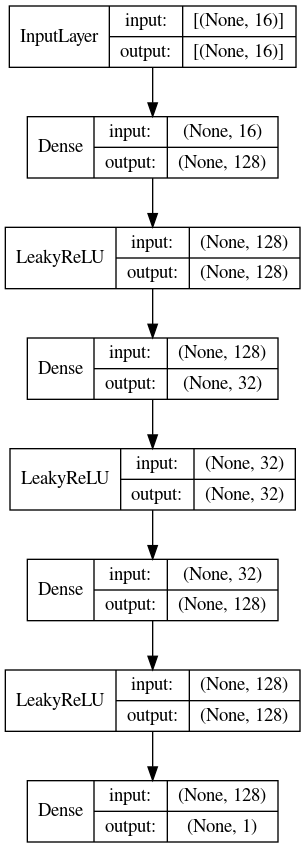
\includegraphics[width=.4\linewidth]{Plots/model_0fj.png}
    \end{subfigure}%
    \begin{subfigure}{.5\textwidth}
      \centering
      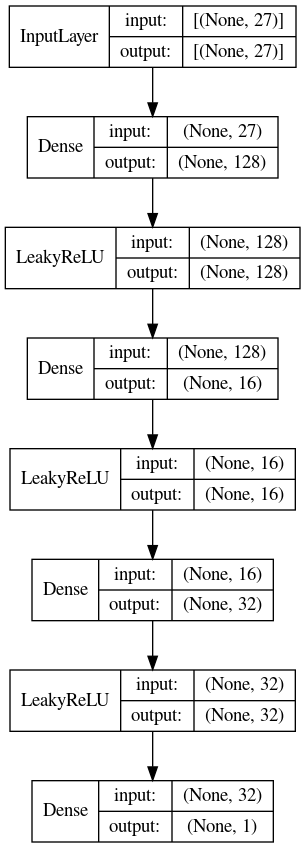
\includegraphics[width=.4\linewidth]{Plots/model_1fj.png}
    \end{subfigure}
    \caption{Visualization of the NN architecture for the zero forward jet region (left) and the $\geq 1$ forward jets region (right).}
    \label{fig:models}
\end{figure}

\section{Input features for the neural network}
\label{sec:inputfeatures}

For the $tq\gamma$ process, it is not easy to find characteristic variables that distinguish this process from background processes. 
This is due to the small $S/B$ ratio of the process and the similarity of some background processes. 
A different neural network based approach was used to find features that have the most discriminatory power. 

The final input features used for the two NN models for discrimination are listed in Table \ref{tab:features0} and \ref{tab:features1} for the $0\, fj$ and $\geq 1\, fj$ regions respectively.

\begin{table}
    \centering
    \begin{tabular}{c|c|c}
        \toprule
        {} &                     $0\, fj$ variables & Explanation\\
        \midrule
        0  &                                HT &  Scalar sum of all trasnverse momenta\\ \hline
        1  &                           blep\_dr & $\Delta R$ of $b$-jet and lepton\\ \hline
        2  &                            bph\_pt & Transverse momentum of photon+$b$-quark\\ \hline
        3  &                           lbj\_eta & $|\eta|$ of leading $b$-jet\\ \hline
        4  &                            lbj\_pt & $p_T$ of leading $b$-jet\\ \hline
        5 &  lbj\_tagWeightBin&                  \\
        &\_DL1r\_Continuous &\\\hline
        6  &                          lep1\_eta & $p_T$ of leading lepton\\ \hline
        7  &                           lep1\_id & ID to determine lepton type\\ \hline
        8  &                          lepph\_dr & $\Delta R$ distance between lepton and photon\\ \hline
        9  &                           met\_met & Missing transverse energy\\ \hline
        10 &                            ph\_eta & $\eta$ of the photon\\ \hline
        11 &                             ph\_pt & $p_T$ of the photon\\ \hline
        12 &                             top\_m & invariant mass of top quark\\ \hline
        13 &                          topph\_pt & Summed $p_T$ of top quark and photon\\ \hline
        14 &                       transMassWb & transverse mass of lepton, $b$-jet and neutrino\\ \hline
        15 &                      transMassWph & transverse mass of photon and W boson\\ 
        \bottomrule
        \end{tabular}
    \caption{Input variables of the NN for events with no forward jets alongside their explanation.}
    \label{tab:features0}
\end{table}
\begin{table}
    \centering
    \begin{tabular}{c|c|c}
        \toprule
        {} &                     $\geq 1\, fj$ variables & Explanation\\
        \midrule
        0  &                                HT  & See Table \ref{tab:features0} \\\hline
        1  &                            Wbsn\_e & Energy of W boson\\\hline
        2  &                             bfj\_m & Invariant mass of $b$-jet and forward jet\\\hline
        3  &                           blep\_dr & See Table \ref{tab:features0}\\\hline
        4  &                            blep\_m & Invariant mass of $b$-jet and lepton\\\hline
        5  &                             bph\_m & Invariant mass of $b$-jet and photon\\\hline
        6  &                            fj\_eta & $|\eta|$ of forward jet\\\hline
        7  &                            fj\_phi & $\phi$ of forward jet\\\hline
        8  &                         fjet\_flag & forward jet is jet with highest $p_T$ in event\\\hline
        9  &                       fjph\_ctheta & $cos(\theta)$ between photon and forward jets\\\hline
        10 &                         fjph\_deta & Distance in $|\eta|$ between forward jet and photon\\\hline
        11 &                           fjph\_dr & $\Delta R$ distance between forward jet and photon\\\hline
        12 &                            fjph\_e & Energy of forward jet and photon\\\hline
        13 &                            fjph\_m & Invariant mass of forward jet and photon\\\hline
        14 &                           lbj\_eta & See Table \ref{tab:features0}\\\hline
        15 &                           lbj\_phi & $\phi$ of leading $b$-jet\\\hline
        16 &                            lbj\_pt & See Table \ref{tab:features0}\\\hline
        17 &  lbj\_tagWeightBin&                  See Table \ref{tab:features0}\\
        &\_DL1r\_Continuous &\\\hline
        18 &                          lep1\_eta &See Table \ref{tab:features0}\\\hline
        19 &                           lep1\_pt &$p_T$ of leading lepton\\\hline
        20 &                           met\_met &See Table \ref{tab:features0}\\\hline
        21 &                           met\_phi &$\phi$ of missing transverse momentum\\\hline
        22 &                            ph\_phi &$\phi$ of photon\\\hline
        23 &                             ph\_pt &See Table \ref{tab:features0}\\\hline
        24 &                             top\_m &See Table \ref{tab:features0}\\\hline
        25 &                      topph\_ctheta &$cos(\theta)$ between top quark and photon\\\hline
        26 &                       transMassWb  &See Table \ref{tab:features0}\\\hline
        \bottomrule
    \end{tabular}
    \caption{Input variables of the NN for events with at least one forward jet alongside their explanation.}
    \label{tab:features1}
\end{table}


\section{Performance and distribution of the NN output}
The distribution of the NN output for $\geq 1\text{-}fj$ is displayed in Figure \ref{fig:NNdistro}. In this plot, the contributions from different signal and background MC samples are shown and stacked on top of each other. The data samples are viewed seperately and also added to the plot. 
These plots confirm that the $S/B$ ratio is larger in bins with higher NN output values.  \\ 
To determine the performance of the NN output, background suppression is plotted against the signal efficiency at different cut values on the NN output in a receiver operating characteristic (ROC) curve in Figure \ref{fig:rocfull}. 
The signal efficiency (SE) is calculated as follows: 
\begin{align*}
    SE = \frac{\text{Number of true signal events }}{\text{Total number of signal events}}
\end{align*}
and the background suppression (BS) is calculated with the formula
\begin{align*}
    BS = 1 - \frac{\text{Number of true background events }}{\text{Total number of background events}}
\end{align*}




\begin{figure}
    \centering
    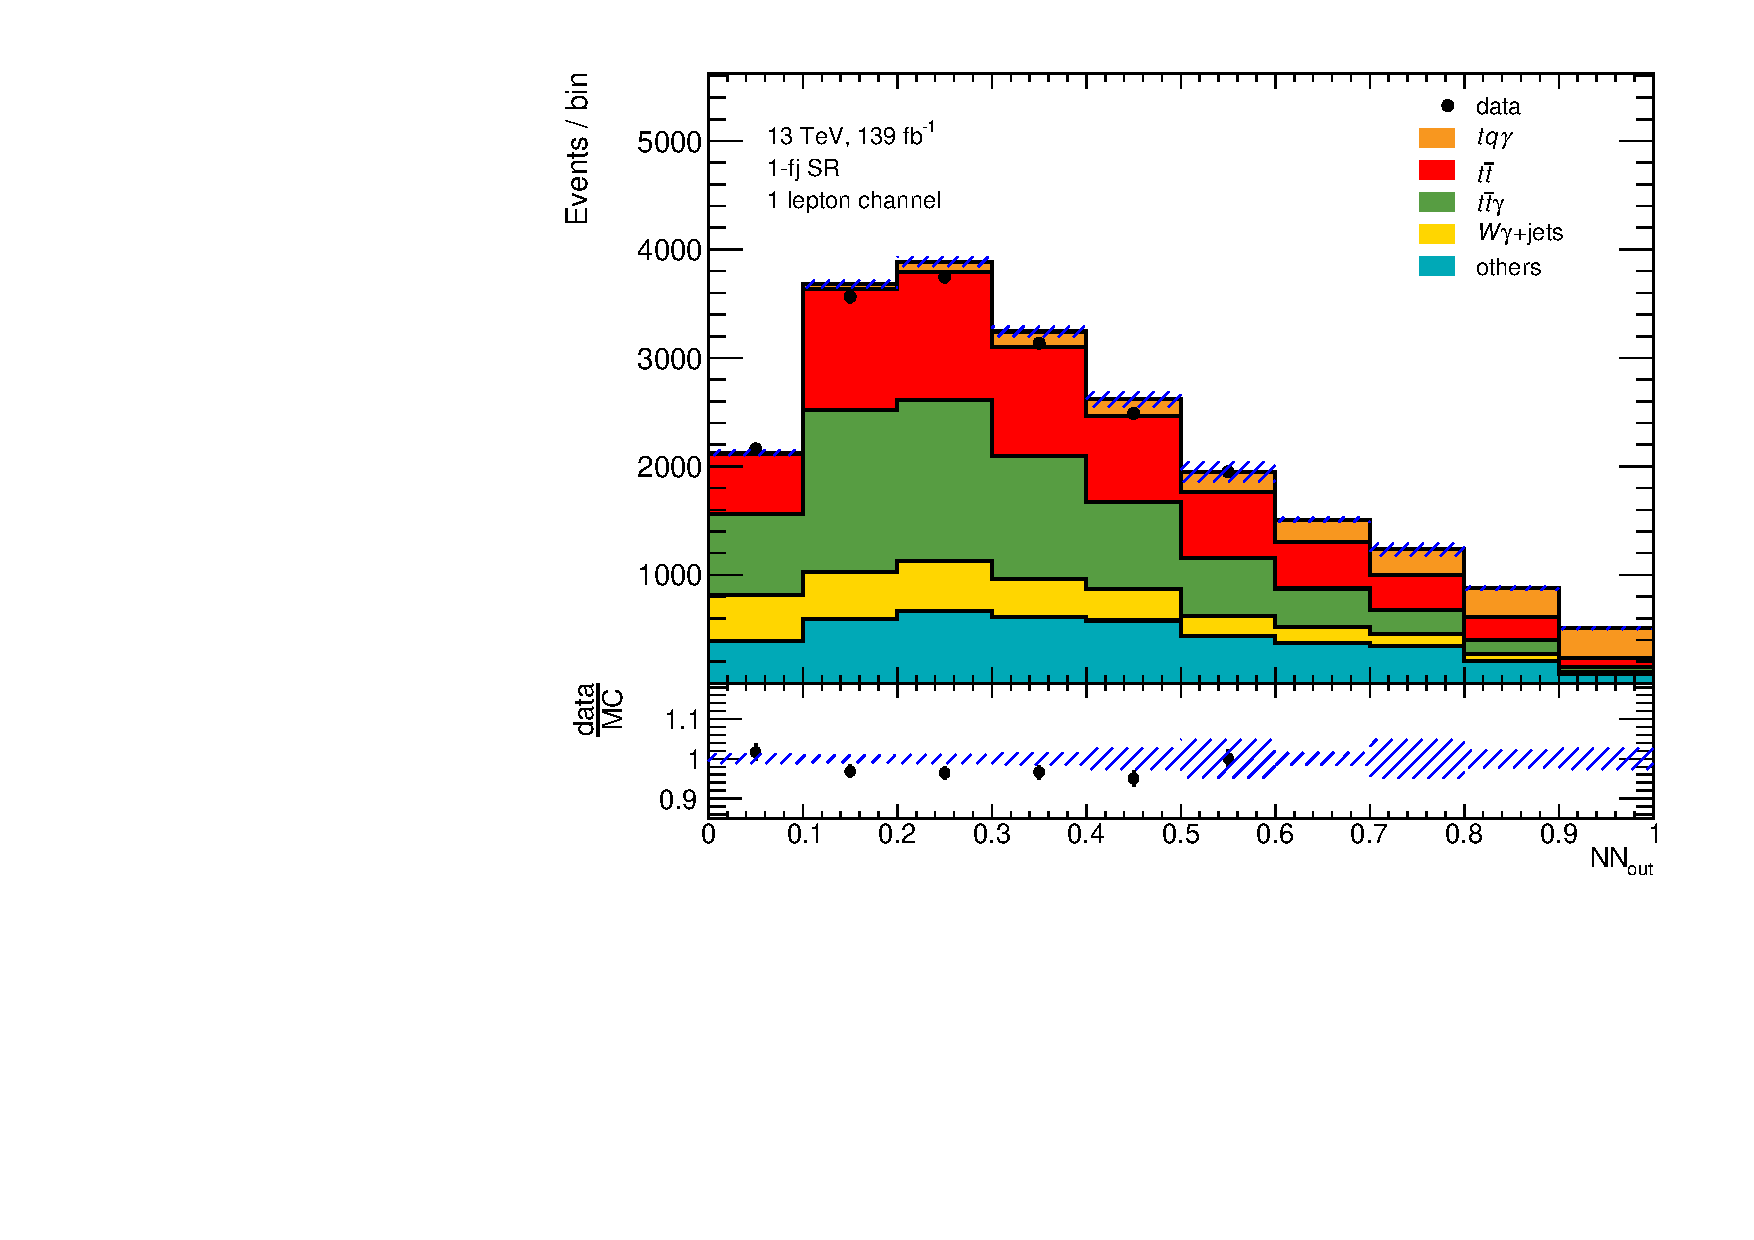
\includegraphics[width=0.8\textwidth]{Plots/NN_out_mix_GANZ.pdf}
    \caption{Visualisation of the NN output event distribution.}
    \label{fig:NNdistro}
\end{figure}
\begin{figure}
    \centering
    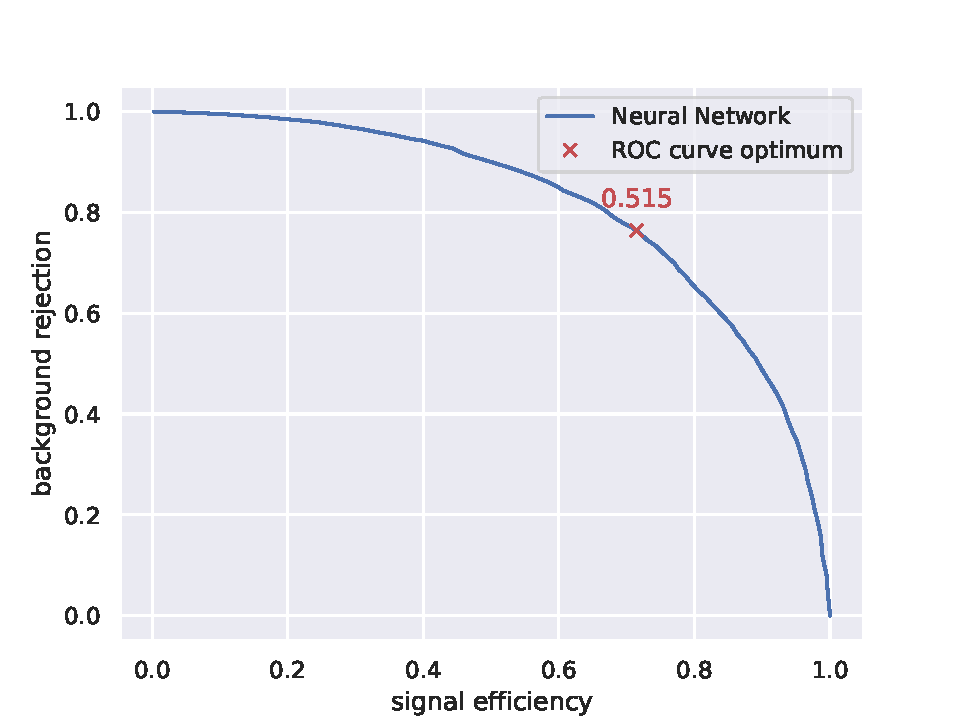
\includegraphics[width=0.5\textwidth]{Plots/ROC-Curve-fullt.pdf}
    \caption{ROC curve of the neural network with the point of maximized signal efficiency and backgrund rejection, which is the closest data point to the (1,1) corner.}
    \label{fig:rocfull}
\end{figure}

